\section{Tools}
\subsection{Jupyter}
The Jupyter Notebook is an open-source web application that supports data cleaning and transformation, numerical simulation, statistical modeling, data visualization, machine learning, etc. by allowing us to create and share documents that contain live code, equations, visualizations and narrative text. Jupyter allows for displaying the result of computation inline in the form of rich media (SVG, LaTeX, etc.). The Jupyter notebook combines two components:
\begin{itemize}
  \item \textbf{A web application}: a browser-based tool for interactive authoring of documents which combine explanatory text, mathematics, computations and their rich media output.
  \item \textbf{Notebook documents}: a representation of all content visible in the web application, including inputs and outputs of the computations, explanatory text, mathematics, images, and rich media representations of objects.
\end{itemize}
Jupyter notebook is gaining rapid popularity in the field of data science for making sharing documentation and codes for replication very easy. In this project, the codes are written in python notebook which can be accessed from http://github.com/.

\subsection{Tensorflow}
TensorFlow\textsuperscript{TM} is an open source software library developed within Google’s AI organization by the Google Brain team with a strong support for machine learning and deep learning. Its flexible architecture allows easy deployment of computation across a variety of platforms (CPUs, GPUs, TPUs), and from desktops to clusters of servers to mobile and edge devices. It is being used at a number of well known companies like Uber, Google, AMD, etc. for high performance numerical computation and machine learning. While TensorFlow is capable of handling a wide range of tasks, it is mainly designed for deep neural network models. It will serve as baseline to test the metamorphic relations identified in section \ref{MRused}.

\section{Algorithm}
\subsection{Convolutional neural network}
\subsection{2-layer neural network}

\section{Dataset}
\subsection{MNIST Dataset}
The MNIST database of handwritten digits maintained by Yann LeCun \cite{MNIST}, has a training set of 55,000 examples, and a test set of 10,000 examples. It is a subset of a larger set available from NIST. The digits have been size-normalized and centered in a fixed-size image. It is a good database for people who want to try learning techniques and pattern recognition methods on real-world data while spending minimal efforts on preprocessing and formatting. The MNIST database was constructed from NIST's Special Database 3 and Special Database 1 which contain binary images of handwritten digits. The original black and white (bilevel) images from NIST were size normalized to fit in a 20x20 pixel box while preserving their aspect ratio. The images were centered in a 28x28 image by computing the center of mass of the pixels, and translating the image so as to position this point at the center of the 28x28 field.

\subsection{EMNIST Dataset}
The EMNIST dataset is a set of handwritten character digits derived from the NIST Special Database 19
and converted to a 28x28 pixel image format. The EMNIST dataset structure directly matches the MNIST dataset.

\subsubsection{Dataset Summary}
There are six different splits provided in this dataset. A short summary of the dataset is provided below:
\begin{itemize}
  \item EMNIST ByClass: 814,255 characters. 62 unbalanced classes.
  \item EMNIST ByMerge: 814,255 characters. 47 unbalanced classes.
  \item EMNIST Balanced:  131,600 characters. 47 balanced classes.
  \item EMNIST Letters: 145,600 characters. 26 balanced classes.
  \item EMNIST Digits: 280,000 characters. 10 balanced classes.
  \item EMNIST MNIST: 65,000 characters. 10 balanced classes.
\end{itemize}
The full complement of the NIST Special Database 19 is available in the ByClass and ByMerge splits. The EMNIST Balanced dataset contains a set of characters with an equal number of samples per class.
The EMNIST Letters dataset merges a balanced set of the uppercase and lowercase letters into a single 26-class task. The EMNIST Digits and EMNIST MNIST dataset provide balanced handwritten digit datasets directly compatible with the original MNIST dataset.

\begin{figure}[htb!]
        \centering
        \begin{subfigure}[b]{\textwidth}
            \centering
            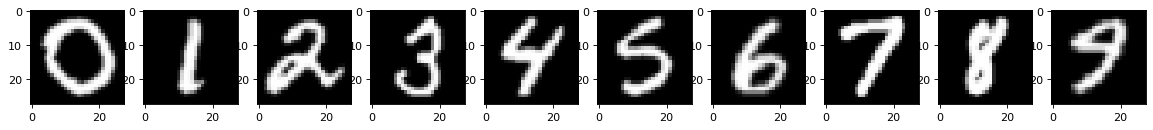
\includegraphics[width=\linewidth]{images/digit.png}
            \caption{Sample EMNIST-MNIST dataset}
            \label{fig:EMNIST MNIST dataset}
        \end{subfigure}%
        \label{fig:Rotate-misclassifications}
        \begin{subfigure}[b]{\textwidth}
            \centering
            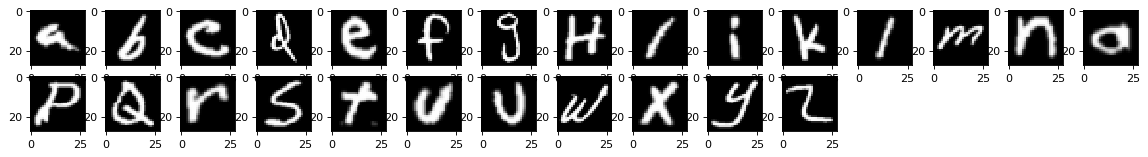
\includegraphics[width=\linewidth]{images/letter.png}
            \caption{Sample EMNIST-MNIST dataset}
            \label{fig:EMNIST MNIST dataset}
        \end{subfigure}%
        \label{fig:Rotate-misclassifications}
    \end{figure}
    \FloatBarrier

    
\subsection{Fashion MNIST Dataset}
Fashion-MNIST is a dataset of Zalando's article images—consisting of a training set of 55,000 examples and a test set of 10,000 examples. Each example is a 28x28 grayscale image, associated with a label from 10 classes. 

\begin{table}[ht]
\centering
\begin{tabular}{|c|c|}
\hline
\textbf{Label} & \textbf{Description} \\ \hline
0  &   T-shirt/top \\ \hline
1  &   Trouser \\ \hline
2   &	Pullover \\ \hline
3   &	Dress \\ \hline
4   &	Coat \\ \hline
5   &	Sandal \\ \hline
6   &	Shirt \\ \hline
7   &	Sneaker \\ \hline
8   &	Bag \\ \hline
9   &	Ankle boot \\ \hline
\end{tabular}
\caption{Data file format.}
\label{tbl:training-file-format}
\end{table}

\begin{figure}[htb!]
        \centering
        \begin{subfigure}[b]{\textwidth}
            \centering
            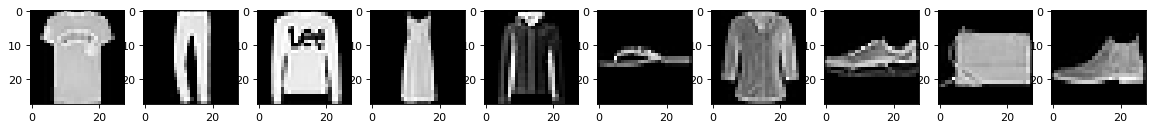
\includegraphics[width=\linewidth]{images/fashion.png}
            \caption{Sample EMNIST-MNIST dataset}
            \label{fig:EMNIST MNIST dataset}
        \end{subfigure}%
        \label{fig:Rotate-misclassifications}
    \end{figure}
    \FloatBarrier
    
\subsection{Format of Dataset}
The data is stored in a very simple file format designed for storing vectors and multidimensional matrices. All the integers in the files are stored in the MSB first (high endian) format used by most non-Intel processors. There are 4 files:
\begin{itemize}
  \item train-images-idx3-ubyte: training set images
  \item train-labels-idx1-ubyte: training set labels
  \item t10k-images-idx3-ubyte:  test set images
  \item t10k-labels-idx1-ubyte:  test set labels
\end{itemize}
The format of training and test files are described in the following table.
\begin{table}[ht]
\centering
\begin{tabular}{|c|c|c|c|}
\hline
\textbf{offset} & \textbf{type}    &      \textbf{value}    &      \textbf{description} \\
\hline
0000  &   32 bit integer & 0x00000801(2049) & magic number (MSB first) \\
\hline
0004  &   32 bit integer & 60000       &     number of items \\
\hline
0008  &   unsigned byte  & ??          &     label \\
\hline
0009  &   unsigned byte  & ??          &     label \\
\hline
\multicolumn{4}{|c|}{\textbf{........}} \\
\hline
xxxx  &   unsigned byte  & ??          &     label \\
\hline
\multicolumn{4}{|c|}{\textbf{The label values are 0 to 9.}} \\
\hline
\end{tabular}
\caption{Training data file format.}
\label{tbl:training-file-format}
\end{table}

\begin{table}[ht]
\centering
\begin{tabular}{|c|c|c|c|}
\hline
\textbf{offset} & \textbf{type}    &      \textbf{value}    &      \textbf{description} \\
\hline
0000  &   32 bit integer & 0x00000803(2051) & magic number (MSB first) \\
\hline
0004  &   32 bit integer & 60000       &     number of images \\
\hline
0008  &   unsigned byte  & 28          &     number of rows  \\
\hline
0012  &   unsigned byte  & 28          &     number of columns \\
\hline
0016  &   unsigned byte  & ??          &     pixel \\
\hline
0017  &   unsigned byte  & ??          &     pixel \\
\hline
\multicolumn{4}{|c|}{\textbf{........}} \\
\hline
xxxx  &   unsigned byte  & ??          &     pixel \\
\hline
\multicolumn{4}{|c|}{\textbf{
\shortstack{Pixels are organized row-wise. Pixel values are 0 to 255. \\ 0 means background (white), 255 means foreground (black).}}} \\
\hline
\end{tabular}
\caption{Test data file format.}
\label{tbl:test-file-format}
\end{table}



% \subsection{Docker}
% For replication of results. Image can be downloaded from dockerhub. Attached volume for persisting data.


